\documentclass[a4paper,12pt]{article}
\usepackage{amsmath}
\usepackage{amssymb}
\usepackage{graphicx}
\usepackage{siunitx}
\usepackage[hidelinks]{hyperref}



\begin{document}
\title{An Automatic Landing System for UAVs: Progress Report}
\author{By: James Duley, \texttt{james.duley@canterbury.ac.nz}, 28245623\\Supervisors: Kelvin Barnsdale and Masako Kishida}
\maketitle
\thispagestyle{empty}
\newpage
\begin{abstract}
	The goal of the project is to construct an optical navigation aid for a UAV that it can use in GPS denied environments. The project will use a single board computer with a camera and inertial measurement unit to do real-time inertially-aided monocular simultaneous localisation and mapping. 
	Hardware selection has been made and fictitious sensor data has been created for use with testing.
\end{abstract}
\newpage

\pagenumbering{roman}
\tableofcontents
\newpage

\pagenumbering{arabic}

\section{Project Overview\label{sec:overview}}
\subsection{Group Goals}
The University of Canterbury Electrical and Computer Engineering Department has been contracted by the Defence Technology Agency (DTA) to develop a number of components of an autonomous unmanned aerial vehicle (UAV) landing system. The DTA is ``the main provider of research, science and technology to support the New Zealand Defence Force and the Ministry of Defence''. They have developed a number of UAVs for which they want to add some autonomous behaviour in GPS denied environments.

Two goals were chosen by the group for this project, they are to develop:
\begin{itemize}
	\item A precision glide path radio guidance system for use when landing a fixed wing UAV.
	\item A optical navigation aid for supplementing an intermittent GPS signal.
\end{itemize}
Three of the four students will develop the former and the author will develop the latter and will be the subject of this report.

\subsection{An Optical Navigation Aid}
The goal of the author is to construct a working prototype of a standalone optical navigation aid that the DTA can use on their UAVs. This should be demonstrated by a test flight at the end of the project.

The system is should meet the following specifications:
\begin{itemize}
	\item The system should return six degree of freedom information for use by the flight controller, that is, location and orientation relative to the starting point.
	\item The location should be accurate to within 10\% of the length of the shortest path to the staring point within the tracks travelled by the UAV.
	\item The orientation should be accurate to 1 degree.
	\item The system should not be lager than \SI{0.00025}{m^{3}}.
	\item The system should not cost more than \$150 to produce.
\end{itemize}

\section{Progress to Date\label{sec:progress}}
\subsection{Approach Evaluation}
\subsubsection{Motivation\label{motivation}}
Unmanned Aerial Vehicles (UAVs) typically rely on GPS for navigation, however, there are situations when this is not feasible, such as, indoors and when there is high interference. One option for navigating in such a situation is using an optical sensor. There are two main forms an optical navigation aid can take, they are:
\begin{itemize}
	\item Pure optical flow. 
	\item Visual simultaneous localisation and mapping (SLAM).
\end{itemize}

\subsubsection{Pure Optical Flow}
Pure optical flow systems generally use a low resolution sensor and return a mean two-dimensional pixel flow this is then combined with range finding device and a three-axis gyro to give ground velocities, attitude change rates and height above the ground. Robust solutions have already been implemented and are available for purchase\cite{honegger2013open}.

This solution has the following pros:
\begin{itemize}
	\item Robust solutions already exist.
\end{itemize}
It also has the following cons:
\begin{itemize}
	\item Gives velocities that need to be integrated for absolute distances which is prone to accumulative error.
	\item Altitude limited by the range finding component, typically well under \SI{100}{m}.
\end{itemize}

\subsubsection{Visual SLAM}
Visual SLAM can use depth sensing cameras such as stereo vision, time of flight camera, structured light etc., however, these all have limited distance so only monocular visual SLAM is considered. Monocular visual SLAM uses a single camera and picks out features in each frame. The relative motion of these features between frames is then used to create a three-dimensional point cloud of these features and the path of the camera relative to them. The accuracy of this method can be significantly increased by using the additional information from a gyro. A number of people have implemented such solutions\cite{weiss2011monocular,chowdhary2013gps} but no robust standalone systems exist at the moment.

This solution has the following pros:
\begin{itemize}
	\item Unlimited altitude.
\end{itemize}
It also has the following cons:
\begin{itemize}
	\item Prone to accumulative error, but not like pure optical flow.
	\item More computing power required.
	\item Potentially more expensive as accuracy will depend on the quality of the camera.
\end{itemize}

\subsubsection{Proposed System\label{system}}
The only solution worth implementing for this project is visual SLAM. This is because it offers the best performance potential and because no work needs to be done on pure optical flow.

The system will use the following three pieces of hardware:
\begin{itemize}
	\item A single board computer (SBC).
	\item An inertial measurement unit (IMU).
	\item A camera.
\end{itemize}


\subsection{Completed Tasks}
\subsubsection{Hardware Selection}
The first task completed was hardware selection. A number of options were looked at for each component and the cheapest that appeared to be sufficient for the project were selected.

The proposed SBC is an ODROID-U3 as it provides good performance for its price. It costs 65USD and can communicate with the IMU via I2C and with the flight controller via UART.

The proposed IMU could be any number of devices but the Invensense MPU-9150 presents good value for a 9 degrees of freedom sensor which is available in a convenient breakout board that can be used for this project. It costs 15USD.

The camera is much harder to choose but ideally a machine vision camera with a global shutter which implements the IIDC standard or the UVC standard should suffice. Initially a cheap CMOS webcam will be used as the author has one already, however, a number of other specific webcams will be more suitable. The Xbox Live Vision camera has a CCD sensor and hence global shutter and can be acquired for approximately \$20. The PlayStation Eye camera is another camera that could be useful as it can be modified to use an external trigger ensuring accurate synchronization of the camera and IMU. It has a CMOS sensor with rolling shutter, however, so this may not be ideal. It can also be acquired for approximately \$20. The ideal camera for this project is the Point Grey Firefly MV which is a machine vision camera, it is significantly more expensive unfortunately, costing 275USD.

\subsubsection{Data Simulation}
The second task completed was the construction of some fictitious data to test the future code. This consisted of creating camera view points of a large image
 laid on the ground plane with matching pose data. This is what the camera would record if the UAV were flown over such a ground plane. This was done using the basic pinhole camera model and deriving the perspective transform associated with camera being in a certain position and orientation relative to the ground plane. Application of the perspective function was performed using a method in OpenCV (a computer vision library).

 The implementation allows the input of any image to be used as the ground plane and any path for the camera to generate the sequence of frames. This will be very useful for testing the visual SLAM code as it will unambiguously show if it is not working correctly.
\section{Remaining Tasks\label{method}}
To achieve the desired goal an number of steps remain to be undertaken, they are:
\begin{enumerate}
	\item Write visual SLAM code and check if it gives correct results.
	\item Record some real data from a UAV using a GPS and test the code on that footage.
	\item Implement integration with the flight controller.
	\item Test real system on UAV.
	\item Implement other features, such as, loop closure, collision warning, etc., (if time permits).
\end{enumerate}

The Gantt chart in Figure \ref{fig:gantt} shows the proposed time-line for the rest of the project.
\begin{figure}[h]
	\centering
	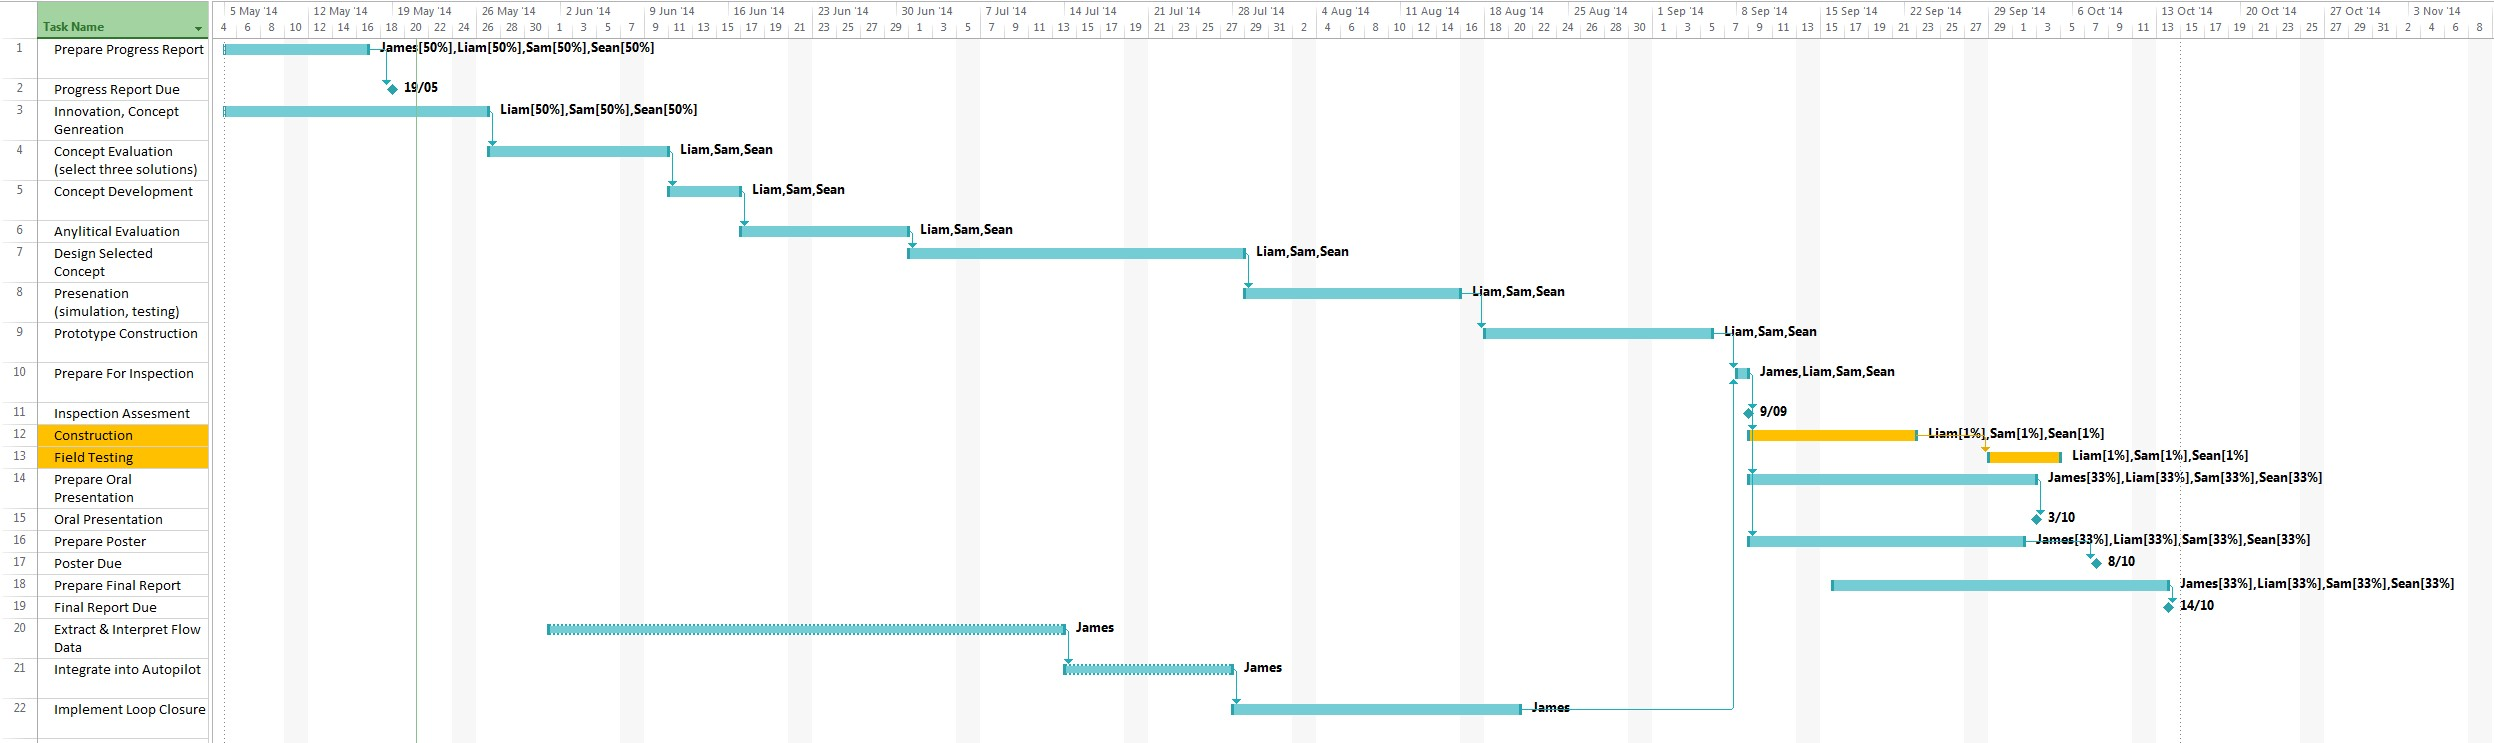
\includegraphics[width=1.45\textwidth, angle=270]{ganttchart.jpg}
	\label{fig:gantt}
	\caption{Proposed time-line for the rest of the project.}
\end{figure}

\section{Sustainability Analysis}
\subsection{Introduction}
There are three aspects to the triple bottom line of sustainability to consider, they are:
\begin{itemize}
	\item Environmental Impact
	\item Economic Impact
	\item Social Impact
\end{itemize}
How this project affects those aspects stem from the fact that the roles of UAVs are replacing a larger manned aircraft. The following subsections will show that.

\subsection{Environmental Impact}
The use of UAVs impacts favourably to the environment compared to a manned aircraft because of the significantly reduced fossil fuel usage. This is because most are electric and those that are not require very little fuel comparatively because the are much smaller and carry a smaller load.

\subsection{Economic Impact}
The most important positive impact of UAVs is that they reduced costs significantly for many tasks that would otherwise required a manned aircraft such as any observation task like aerial searching and filming.

\subsection{Social Impact}
UAVs have a positive social impact because they allow humans to do a number of things more easily, but more importantly, safely. This includes flying into any dangerous environments that would normally put a pilot at risk.

\section{Budget Summary}
This project requires nothing to be bought for it as the author already has the components, or can borrow them. The summary of the costs of the system are shown in Table \ref{tab:budget}.
\begin{table}[h]
	\centering
	\begin{tabular}{| l | l |}

	\hline
	Component & Cost \\
	\hline \hline
	ODROID-U3 & \$76 \\
	\hline
	Invensense MPU-9150 & \$15 \\
	\hline
	USB camera & \$20 \\
	\hline \hline
	Total & \$111 \\ 
	\hline
	\end{tabular}
	\label{tab:budget}
	\caption{Budget}
\end{table}


\bibliography{cv.bib}
\bibliographystyle{unsrt}
\end{document}
